\usepackage[english] {babel}
\usepackage[T1]      {fontenc}
\usepackage{hyperref}

\usepackage{amsmath, amsfonts, graphicx}
\usepackage{tikz}
\usepackage{csquotes}


\setbeamersize
  {text margin left=1em, text margin right=1em}

\title
  [Scoring an SDO]
  {Scoring a Software Development Organization\\ with a Single Number}

\author
  [Ryan]
  {Ryan M. Swanstrom}

\date
  {April 6, 2015}

\institute[SDSU]
  {South Dakota State University}

\begin{document}

\maketitle

\subsection{About Ryan}
\begin{frame}
  {Ryan M. Swanstrom}
  
  \begin{enumerate}
    \item Professional Software Engineer
    \item Blogger/Data Scientist
    \begin{enumerate}
        \item \href{http://101.datascience.community}{Data Science 101 Blog}
        \item Guest Blogger for \href{http://www.datakind.org/blog/}{DataKind}
    \end{enumerate}
    \item Many Other Things
    \item Started this PhD thing in 2006
  \end{enumerate}
\end{frame}

\begin{frame}{Overview}

  \tableofcontents

\end{frame}

\section{Overview and Background}

    \subsection{Software Development Organization}
    
        \begin{frame}{Software Development Organization (SDO)?}
            \begin{displayquote}
                 A \textbf{Software Development Organization (SDO)} is any
                 organization or subset of an organization that is 
                 responsible for the creation, deployment, and 
                 maintenance of software. 
            \end{displayquote}
        \end{frame}
        
    \subsection{Software Engineering}
        \begin{frame}{Software Engineering?}
            \begin{displayquote}
                 \textbf{Software} is not just the
                    programs but also all associated documentation and 
                    configuration data which is
                    needed to make these programs operate correctly
                    \cite{Sommerville2001}
            \end{displayquote} 
            
            \begin{displayquote}
                \textbf{Software Engineering} is the application 
                of a systematic, disciplined, quantifiable
                approach to the development, operation, and maintenance of software
                \cite{Ieee1990} 
            \end{displayquote} 
        \end{frame}
    
    \subsection[SDLC]{Software Development Life Cycle}
        \begin{frame}{Software Development Life Cycle (SDLC)?}
            \begin{figure}[ht]
                \centering
                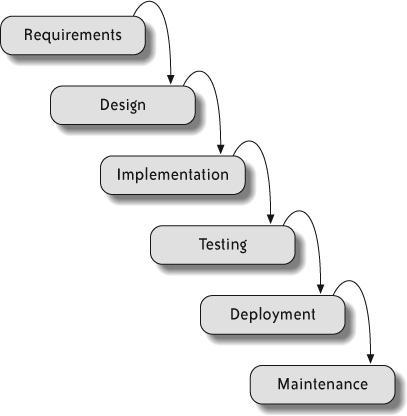
\includegraphics[scale=.86]{images/waterfall.png}
                \caption{SDLC, adapted from \cite{Hibbs2009} }
            \end{figure}
        \end{frame}
    
    \subsection{The Problem}
        \begin{frame}{So What is Wrong?}
            \begin{itemize}
                \item Performance is difficult to measure
                \item Inconsistent
                \item Complicated
                \item Overwhelming
            \end{itemize}
        \end{frame}
    
\section{CRI}

    \subsection{CRI Overview}
    \subsection{Quality}
    \subsection{Availability}
    \subsection{Satisfaction}
    \subsection{Schedule}
    \subsection{Requirements}
    \subsection{Overall}

    \subsection{Comparison}
    
    \subsection{Storage Framework}
        \begin{frame}{SDLC-AE}
            \begin{figure}[ht]
                \centering
                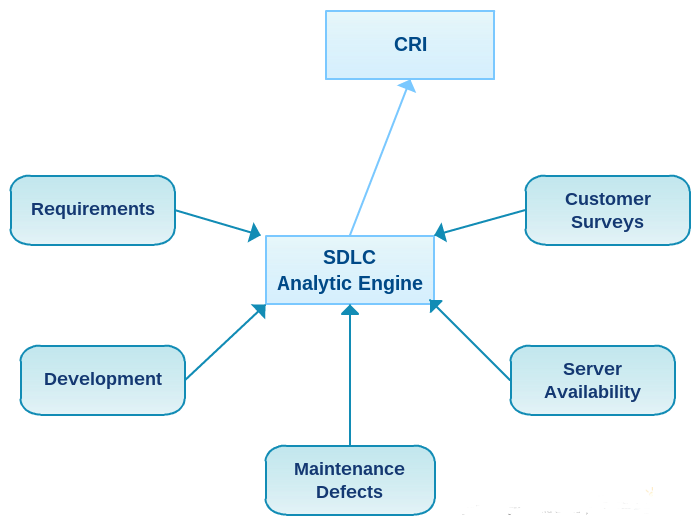
\includegraphics[scale=.5]{images/sdlcae.png}
            \end{figure}
        \end{frame}

\section{Case Study}
    \subsection{Quality}
    \subsection{Availability}
    \subsection{Schedule}
    \subsection{Requirements}
    \subsection{Overall}

\section{Conclusion}

    \subsection{Questions}
        \begin{frame}{Feedback}
            \center 
            Thanks for attending
            
            Questions / Thoughts
          
        \end{frame}

    \subsection{References}
        \begin{frame}{References}
            \bibliographystyle{acm}
            \bibliography{references}
          
        \end{frame}















\begin{frame}{Performance?}
  \begin{itemize}
      \item How is your organization performing?
      \item Compared to last month/year?
  \end{itemize}
\end{frame}

\begin{frame}{What to track?}
  \begin{itemize}
      \item What would you track?
      \item What is important?
      \item How would you measure that?
      \item Can you score that measurement?
      \item With a \textbf{single number}?
  \end{itemize}
\end{frame}


\subsection{Background}

\begin{frame}{What exists for an SDO?}
  \begin{itemize}
      \item Charts
      \item Metrics
      \item Dashboards
      \item KPIs
      \item Scorecards
  \end{itemize}
\end{frame}

\begin{frame}{Balanced Scorecard}
    Strategic Planning and Management System with measures for the following:
    
    \begin{itemize}
      \item Financial 
      \item Customer Focus
      \item Environment/Community
      \item Internal Process
      \item Employee Satisfaction
      \item Learning and Growth
    \end{itemize}
\end{frame}

\subsection{The Approach}

\begin{frame}{5 Important Elements}
    What is important to a Software Development Organization?
    
    \begin{enumerate}
        \item Availability 
        \item Quality
        \item Satisfaction
        \item Schedule
        \item Requirements
    \end{enumerate}
\end{frame}

\begin{frame}{CRI}
    \begin{displayquote}
    The CRI is an algorithm to provide a single number score
    for the performance of an SDO.
    \end{displayquote}
    
    \begin{enumerate}
        \item $[-max, max]$
        \item $max$ : best possible performance (perfect)
        \item $-max$ : worst possible performance (all wrong)
        \item $0$ : expected performance
        \item Time Interval
        \item Element CRI
        \item Overall CRI
    \end{enumerate}
\end{frame}

\subsection{How}

\begin{frame}{Process}
    How will this be done?
\end{frame}

\begin{frame}{Process}
    What is the process for computing CRI?
    
    Given the time interval, perform the following:
    
    \begin{enumerate}
        \item Aquire the necessary data
        \item Compute the scores for the 5 elements
        \item Compute the overall CRI score
        \item Store the results
        \item Display/Share the results
    \end{enumerate}
\end{frame}

\subsection{The Algorithms}

\begin{frame}{Availability - Data}
    
    \begin{tabular}{l | r | r}
        \textbf{Column Name} & \textbf{Data Type} &  \\
        
        Application ID & String  & Required \\
        Frequency Date & Date & Required \\
        Uptime & Float & Optional \\
        Scheduled Downtime & Float & Optional \\
        Unscheduled Downtime & Float  & Optional \\
        Percent Uptime & Float & Required \\
        Expected Percent Uptime & Float & Required \\
    \end{tabular}
\end{frame}

\begin{frame}{Availability - Formula}
    
    \begin{displaymath}
       S_{1_i} = \left\{
         \begin{array}{lr}
           \text{where } A_{a_i} \leq A_{e_i} & : \left[ \frac{A_{a_i} - A_{e_i}}{A_{e_i}} \right] \\
           \text{where } A_{a_i} > A_{e_i}  & : \left[ \frac{A_{a_i} - A_{e_i} }{1-A_{e_i}} \right]
         \end{array}
       \right.
    \end{displaymath} 
    \[
        S_1 = \frac{\sum^n_{i=1}S_{1_i}}{n}
    \]

    \begin{itemize}
        \item $A_{a_i}$ actual availability for app i
        \item $A_{e_i}$ expected availability for app i
    \end{itemize}
\end{frame}

\begin{frame}{Quality - Data}
    
    \begin{tabular}{l | r | r}
    \textbf{Column Name} & \textbf{Data Type} &  \\
    
    Application ID & String (factor) & Required \\
    Frequency Date & Date & Required \\
    Development Hours & Integer & Required \\
    Testing Hours & Integer & Optional \\ 
    Defects in SIT & Integer & Optional \\ 
    Defects in UAT & Integer  & Optional \\ 
    Defects in PROD & Integer  & Required \\
    \end{tabular}
\end{frame}

\begin{frame}{Quality - Formula}
    \begin{displaymath}
       S_{2_i} = \left\{
         \begin{array}{lr}
           \text{where } d_i \leq f_i & :  \frac{f_i - d_i}{f_i}  \\
           \text{where } d_i > f_i  & : \frac{f_i-d_i }{6\sigma_i}
         \end{array}
       \right] \text{   , calculate quality score for each app $i$}
    \end{displaymath} 

    \[
        S_{2} = \frac{\sum^n_{i=1} S_{2_i}}{n} \text{   , average the quality scores}
    \]
    \begin{itemize}
        \item $n$ is the number of apps
        \item $d_i$ is the actual number of PROD defects for app $i$
        \item $f$ is the function to predict PROD defects based upon devhours, testinghours, defectsSIT,
            and defectsUAT
        \item $S_{1_i}$ is the quality score for app $i$
        \item $\sigma_i$ estimate of the stan dev of the population using function $f_i$ above
    \end{itemize}
    
\end{frame}

\begin{frame}{Satisfaction - Data}
    
    \begin{tabular}{l | r | r}
        \textbf{Column Name} & \textbf{Data Type} &  \\
        
        Question ID & String  & Required \\
        Question Text & String  & Optional \\
        Application ID & String & Required \\
        Frequency Date & Date & Required \\
        Response & Integer between min and max  & Required \\
        Response Date & Date & Optional \\
    \end{tabular}
\end{frame}

\begin{frame}{Satisfaction - Formula}
    
    \[
        S_3 = \frac{\sum^n_{i=1}\left( \frac{\sum^m_{j=1}a_{ij}- \frac{min + max}{2}}{m}  \right)}{n}
    \]
    
    \begin{itemize}
        \item $a_{i j}$ answer to question $j$ for app $i$
        \item $m$ number of questions
        \item $n$ number of apps
        \item $min$ minimum score for a question
        \item $max$ maximum score for a question
    \end{itemize}
\end{frame}

\begin{frame}{Schedule - Data}
    
    \begin{tabular}{l | r | r}
        \textbf{Column Name} & \textbf{Data Type} &  \\
        
        Application ID & String  & Required \\
        Frequency Date & Date & Required \\
        Scheduled Finish Date & Date & Required \\
        Actual Start Date & Date  & Required \\
        Actual Finish Date & Date  & Required \\
    \end{tabular}
\end{frame}

\begin{frame}{Schedule - Formula}
    
    \begin{itemize}
    \item The best possible score should be achieved
            when meeting the estimated date exactly.
    \item The maximum score
            should come from exactly meeting the estimate.
    \item Given historical
            release data, determine an 
            average $\Delta$ between the actual and the estimated. 
    \item Finishing a project within that $\Delta$ should result 
            in a positive score.
    \item Outside the $\Delta$ results in
            negative scores. 
    \end{itemize}     
              
\end{frame}

\begin{frame}{Requirements - Data}
    
    \begin{tabular}{l | r | r}
        \textbf{Column Name} & \textbf{Data Type} &  \\
        
        Application ID & String  & Required \\
        Frequency Date & Date & Required \\
        Requirements Scheduled & Integer & Required \\
        Actual Requirements Released & Integer  & Required \\
    \end{tabular}
\end{frame}

\begin{frame}{Requirements - Formula}
    \[
        S_5 = \frac{\sum^n_{i=1}\left( R_{a_i} - R_{e_i} \right)}{n}
    \]
    \begin{itemize}
        \item $R_a$ actual requirements completed for application $i$
        \item $R_e$ expected requirements completed for application $i$
    \end{itemize}
\end{frame}

\begin{frame}{Overall CRI}

Weighted average of the 5 elements
    
\[
    CRI =\sum\limits^n_{i=1} w_i S_i \text{  where } \sum\limits^n_{i=1} w_i = 1
\]
\end{frame}

\subsection{Framework}

\begin{frame}{Data Collection Framework}

    \begin{itemize}
        \item Database structure
        \item Queries
        \item Computations
        \item Overall, how to store and compute CRI
    \end{itemize}
\end{frame}

\subsection{Conclusion}

\begin{frame}{Project Goals}
    Upon completion, this work shall identify:
    \begin{itemize}
        \item Define \textbf{What} characteristics should be measured for an SDO
        \item Define \textbf{How} to measure those characteristics
        \item Map the relationship or lack of relationship with a Balanced Scorecard
        \item Create a Framework to store the necessary data for CRI
        \item Outline a Process to generate the CRI score
        \item Provide an example CRI score with real data
    \end{itemize}
\end{frame}



\end{document}
